%Anfoderungsanalyse

%%%%%%%%%%%%%%%%%%%%%%%%
\chapter{Analyse}
\label{sec:Anforderungsanalyse}
%%%%%%%%%%%%%%%%%%%%
Das Konzept der modularen Anlagen eröffnet neue Möglichkeiten, bringt aber auch neue Herausforderungen. Durch die Flexibilität ist es unter anderem denkbar, dass Module öfter ausgetauscht werden.

Welche Informationen stehen zur Verfügung? -> modulare Anlage, PFE (Verweis auf Problemlöseprozess)

Welche Informationen benötigt der Mensch? -> damit dieser Lösung finden und entscheiden kann

Was lässt sich alles anpassen? -> notwendigkeit für Individualisierung?

Interaktionsmechanik -> wieso ist das so wichtig? Welche Einflüsse gibt es? 

\todo{umschreiben}

\section{Use Case}
Der zuständige Mitarbeiter für die Produktionsplanung der modularen Anlage erhält vom Assistenzsystem die Meldung, dass das Modul Temper in spätestens 7 Tagen gewartet werden muss. Um eine geeignete Lösung für die Aufrechterhaltung der Produktion zu finden bestätigt der Mitarbeiter das Problem. Nun gibt das Assistenzsystem die Möglichkeit die Rahmenbedingungen für die Problemlösung festzulegen. Der Hersteller des Temperiermoduls hat die Dauer der Wartung auf zwei Tage festgelegt. Damit das Assistenzsystem nach geeigneten Lösungen suchen kann definiert der Mitarbeiter die Ziele. Da die Produktion zur Zeit gut ausgelastet ist darf die Anlage maximal drei Stunden still stehen. Mit dieser Angabe sucht nun das Assistenzsystem nach Lösungen, die das definierte Ziel einhalten. Es findet folgende Möglichkeiten:
\begin{itemize}
\item \textbf{Modul leihen:} Der Hersteller des Moduls bietet die Möglichkeit für den Zeitraum der Wartung ein Modul mit den gleichen Spezifikationen zu leihen.
\item \textbf{Modul durch zwei Module tauschen:} Um den geforderten Temperaturbereich der Produktion abzudecken können zwei Module eingesetzt werden.
\item \textbf{Wartung aufschieben:} Die Meldung des Moduls wird ignoriert und so weiter produziert, wie bisher.
\end{itemize}
Um dem Mitarbeiter eine entsprechende Entscheidungshilfe zu geben werden die Lösungsmöglichkeiten mit relevanten Fakten versehen. Diese sind in Tabelle \ref{tab:UseCase-Lösungen} dargestellt.

\begin{table}[htbp]
\centering
\begin{tabular}{p{0.16 \textwidth}|p{0.22 \textwidth}|p{0.22 \textwidth}|p{0.22 \textwidth}|}
\textbf{Lösung} & Modul leihen & Modul durch 2 Module tauschen & Wartung aufschieben \\
\hline
\textbf{Stillstand-zeit} & 1 Stunde & 3 Stunden & 0 Stunden \\
\hline
\textbf{Personal-aufwand	} & 2 Mitarbeiter & 3 Mitarbeiter & 0 Mitarbeiter \\
\hline
\textbf{Leihkosten} & 5.000€ & 0€ & 0€ \\
\hline
\textbf{Hinweis} & Lieferzeit des Moduls beträgt aktuell 5 Tage. & & Bei Verschiebung der Wartung verfällt die Garantie sofort! Garantie läuft noch 2 Jahre. \\
\hline
\end{tabular}
\caption{Use Case: Lösungsmöglichkeiten für das Problem}
\label{tab:UseCase-Lösungen}
\end{table}
Diese Fakten werden visuell unterstützt. Im Fall des Modultauschs zeigt das Assistenzsystem an, wo Änderungen im Rezept vorgenommen werden müssen und welche Services sich verändern.

\section{Vorhandene Informationen}
Die modulare Anlage stellt mittels des Module Type Package (MTP) eine Reihe an Informationen zur Verfügung, welche für den Problemlöseprozess verwendet werden können. Zur Visualisierung einiger der Informationen wird die Prozessführungsebene verwendet. In den folgenden Abschnitten sind die Menge und Art der vorhandenen Informationen detailliert beschrieben. 

\subsection{Modulare Anlage}
Der Lebenszyklus einer modulare Anlage wird in unterschiedliche Phasen eingeteilt. Sie besteht aus Planung, Errichtung, Betrieb und Demontage. \cite{Obst2013} \todo{hier ist ein Sprung} Besonderer Augenmerk in dieser Arbeit liegt auf dem Potential der Flexibilität. So kann die modulare Anlage beispielsweise bei Wartungsarbeiten an einem Modul mit einem alternativen Modul weiter betrieben werden.

Probleme können jedoch nicht nur beim Austausch von Modulen entstehen. Es ist auch denkbar, dass ein Service eine Warnung ausgibt. Nun müsste die Ursache gefunden und das Problem gelöst werden. Welche Probleme beim Betrieb der modularen Anlage auftreten können ist in Abschnitt \ref{Probleme-modulare-Anlage} näher beschrieben.

Um diese Probleme lösen zu können, muss unter anderem klar sein, welche Informationen zur Verfügung stehen. Für den Austausch von Informationen zwischen Prozessführungsebene (PFE) und Modul wird das Modul Type Package (MTP) verwendet. Da der Modulhersteller entscheiden kann, welche Informationen zur Verfügung gestellt werden \todo{Zitat}, unterscheidet sich der konkrete Inhalt des MTP von Modul zu Modul. Es soll hier nicht auf den konkreten Aufbau des MTPs eingegangen werden.

\subsubsection*{Informationsaustausch mittels MTP}
Das Modul stellt eine Reihe an Informationen zur Verfügung, die durch das Modul Type Package (MTP) beschrieben sind. Im MTP sind unter anderem das HMI und die Services hinterlegt. \cite{VDI2658-Blatt1}

Für einen eindeutigen Austausch von Informationen sind Schnittstellen definiert. Jede Schnittstellendefinition besteht aus einem Erklärungstext und den spezifischen Informationsvariablen. Da für jede Schnittstelle andere Informationen übertragen werden, sind hier nur allgemeine relevante Aspekte gelistet. So können unter anderem Einheiten, Maximal- und Minimalwerte oder Prozesswerte übermittelt werden. \cite{VDI2658-Blatt3}
\begin{itemize}
\item \textbf{TagName:} Name der repräsentierten Information. 
\item \textbf{TagDescription:} Beschreibung der repräsentierten Information, z.B. Innere Temperatur des Reaktors.
\item \textbf{ScaleSettings:} Das Modul teilt der PFE die möglichen Anzeigegrenzen mit.
\item \textbf{UnitSettings:} Übermittelt die Einheit des übertragenen Werts.
\item \textbf{ValueLimitation:} Das Modul gibt die Sollwertgrenzen für bestimmt Parameter vor.
\item \textbf{Feedback Monitoring:} Gibt die Rückmeldung an die PFE, dass eine Fehlfunktion vorliegt.
\item \textbf{Limit Monitoring:} Mittels der Limit Variablen können Werte für Toleranz-, Warnungs- und Alarmgrenzen festgelegt werden. Das Modul überwacht die Variablen und signalisiert eine Grenzwertüberschreitung.
\end{itemize}

\subsubsection*{Services}
Wie bereits in Abschnitt \ref{2:Modulare-Anlagen} beschrieben, werden Module durch Dienste gesteuert. Jeder Dienst kann 16 verschiedene Zustände annehmen und teilt den aktuellen Zustand der PFE mit. Die PFE kann die Zustandsübergänge Reset, Pause, Resume, Unhold, Stop, Abort und Restart anfordern. Bei kontinuierlichen Fahrweisen können zusätzlich Start und Complete angefordert werden. Des Weiteren wird der Zustandsübergang State Change (SC) durch den vorgelagerten Zustand ausgelöst. Die aktuell verfügbaren Zustandswechsel meldet das Modul zurück.

Dienste haben verschiedene Betriebsarten. Sie werden in Offline, Manual, Automatic External und Automatic Internal eingeteilt. Zudem gehört zu jedem Dienst eine Liste mit dem verwendetem Anlagenequipment \cite{VDI2658-Blatt4}. Diese Information könnte für eine Eingrenzung des Problembereichs verwendet werden.

Sollen Dienste näher spezifiziert werden, ist eine Verwendung von Parametern möglich. Es wird zwischen Konfigurationsparameter, Fahrweisenparametern, Prozesswerten und Reportwerten unterschieden. \cite{VDI2658-Blatt4}
\begin{itemize}
\item \textbf{Konfigurationsparameter:} Werden für grundlegende Einstellung verwendet. Ein Ändern ist nur möglich, wenn der Dienst offline ist. Es können beispielsweise die Grenzwerte nachgelagerter Module hinterlegt werden.
\item \textbf{Fahrweisenparameter:} Sind rezeptrelevant, werden vom Dienst beim Starten und Neustart überprüft und bei Zulässigkeit übernommen. Es wird an die PFE rückgemeldet, ob der Parameter übernommen werden konnte. Beispielhafte Parameter sind Sollwerte, wie Temperatur- oder Durchflussvorgaben und Reglerparameter, wie Verstärkung und Nachhaltezeit.
\item \textbf{Prozesswerte:} Werden kontinuierlich gelesen oder geschrieben und stellen Werte bereit oder erwarten diese. Beispielhaft dafür sind modulübergreifende Verriegelungen.
\item \textbf{Reportwerte:} Zur Nachweis- und Dokumentationspflicht werden die Werte in den Zuständen Completed, Aborted und Stopped gespeichert.
\end{itemize}

\subsubsection*{Probleme in modularen Anlagen}
\label{Probleme-modulare-Anlage}
Da die modularen Anlagen mit Diensten gesteuert werden, ändert sich auch die Art an Problemen, die entstehen und die vom Modulbetreiber behoben werden können. Durch die Dienste wird nur noch ein Problembereich angezeigt. Meldet ein Dienst zurück, dass er nicht erfolgreich durchgeführt werden kann, ist noch nicht eindeutig, wo das Problem liegt. Durch die Anzeige von dazugehörigem Equipment und möglichen Serviceabhängigkeiten kann der Problembereich eingegrenzt werden. Bei Betrieb der modularen Anlage im P2O-Lab der TU Dresden treten laut dem Geschäftsführer derzeit häufig Fehler auf, wenn entsprechende Zuläufe nicht geöffnet werden. So meldet aktuell das Reaktormodul nicht zurück, wenn vergessen wurde die Druckluft anzustellen. Dem Betreiber fällt nur auf, dass das Modul nicht so arbeitet, wie es soll. Wurde beim Temperiermodul vergessen den Zulauf für das Wasser zur Kühlung zu öffnen, so meldet sich dieses erst nach ca. zwei Minuten zurück, dass es zu warm wird.

Neben den Problemen, die sich auf herkömmliche Anlage übertragen lassen, können im Zuge der Flexibilität ganz Neue entstehen. Die Option nicht nur Parameter anzupassen sondern auch Module auszutauschen, eröffnet neue Möglichkeiten und stellt den Modulbetreiber vor neue Herausforderungen. Müller und Urbas \cite{Muller2017} haben diesen Gedanken bereits angestoßen. Aus diesem Grund ist es interessant zu begutachten, welche weiteren Faktoren bei einem Modulaustausch relevant werden können.

\subsection{Prozessführungsebene}
\label{3:PFE}
Das MTP stellt eine Reihe an Informationen zur Verfügung. Welche davon wie angezeigt werden ist Aufgabe der Prozessführungsebene. Für das P2O-Lab der TU Dresden wurde eine solche PFE entwickelt \todo{Zitat}. Diese besteht in Ebene zwei, drei und vier aus vier Bereichen (siehe Bild \ref{pic:Bereiche-PFE}) \todo{Bild neben Text?}. In Ebene eins sind lediglich die KPI, die Navigation und das Rezept sichtbar.
\begin{figure}[htbp]
\centering
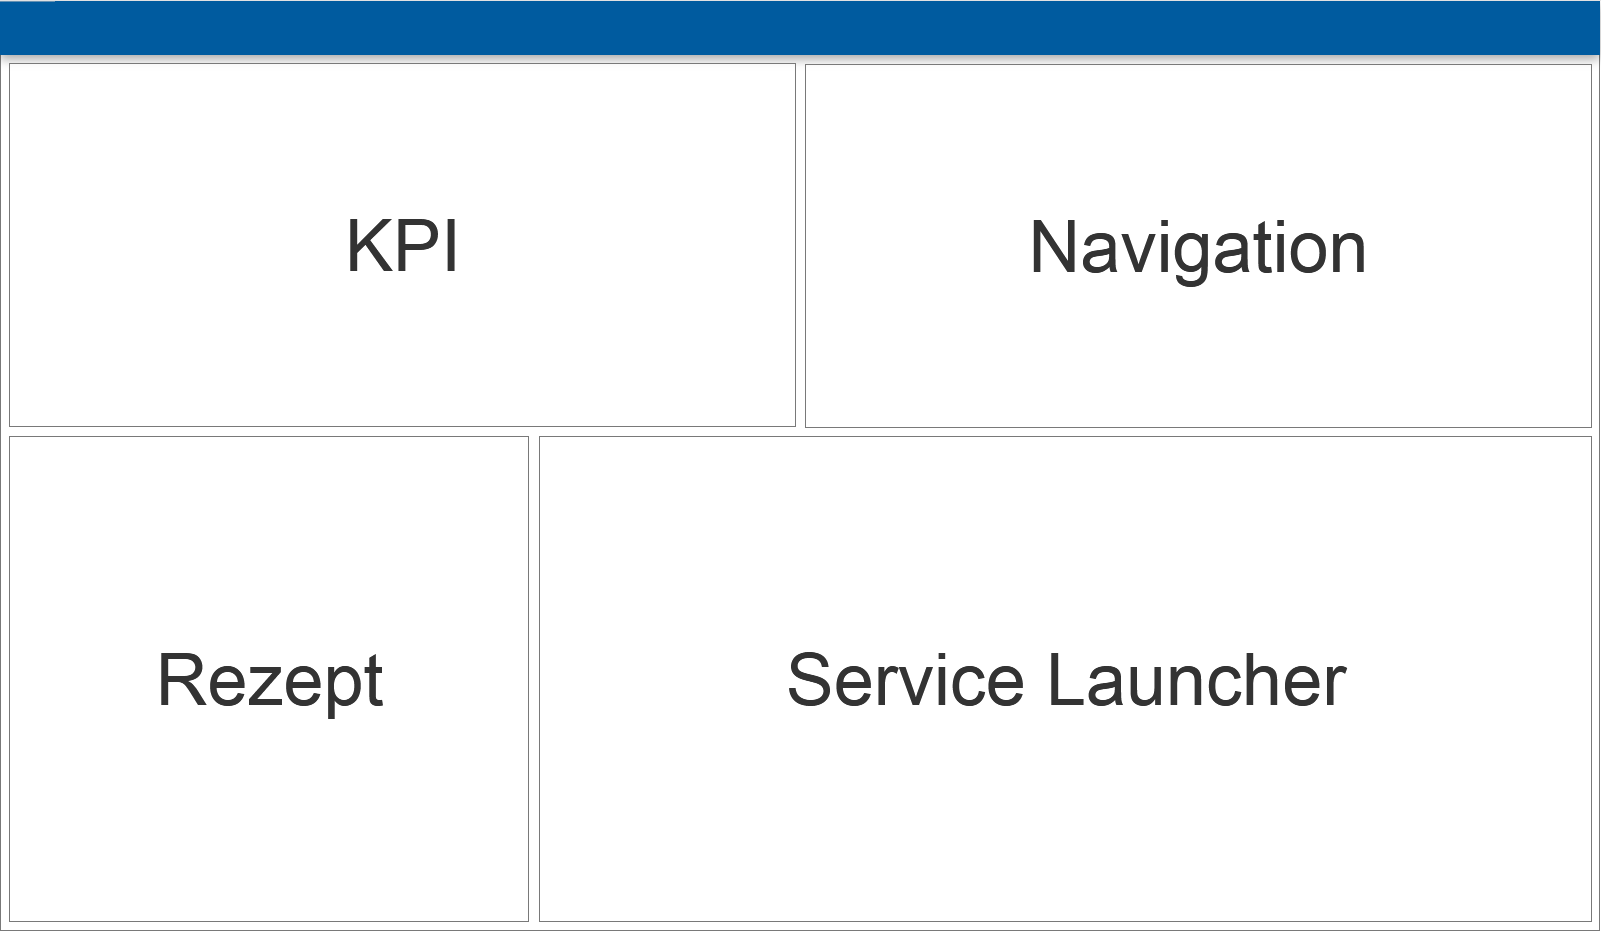
\includegraphics[scale=0.25]{DA_files/Bilder/Analyse/PFE-Bereiche.png}
\label{pic:Bereiche-PFE}
\caption{Die vier Bereiche der PFE}
\end{figure}

\begin{itemize}
\item \textbf{KPI:} Zeigt die KPI der einzelnen Module an.
\item \textbf{Navigation:} Zeigt eine Übersicht über die modulare Anlage an. Durch klicken auf einzelne Module gelangt man zu mehr Details.
\item \textbf{Rezept:} Zeigt das Rezept zur modularen Anlage an. Dieses ist aufgeteilt in Phases, Procedures und Steps (siehe Abschnitt \ref{2:Modulare-Anlagen}).
\item \textbf{Services / HMI:} Zeigt die Dienste der Module an. Diese beinhaltet den aktuellen Zustand und mögliche Zustandsübergänge, die aktuelle Strategie \todo{Fahrweise?} und die aktuelle Betriebsart. Des Weiteren können noch die vorhandenen Fahrweisenparameter angezeigt und eingestellt werden. Auf der letzten Ebene wird statt der Services das HMI des Moduls angezeigt.
\end{itemize}
Für eine besser Übersicht ist die PFE in vier Ebenen eingeteilt. Auf der obersten Ebene ist eine grobe Übersicht über die Anlage gegeben. Die unterste Ebene stellt die meisten Details dar. Tabelle \ref{tab:Ebenen-PFE} beschreibt, welche Informationen auf welcher Ebene dargestellt sind. Mittels der Navigation können die Ebenen gewechselt werden. \todo{Bilder der Ebenen in Anhang}
\begin{table}[htbp]
\centering
\begin{tabular}{p{1,7cm}|p{2,3cm}|p{2,2cm}|p{2,2cm}|p{2,3cm}|}
 & \textbf{Navigation} & \textbf{KPI} & \textbf{Rezept} & \textbf{Services / HMI} \\
\hline
\textbf{Ebene 1} & Shopfloor: Übersicht über alle vorhandenen Anlagen & & Phases für die angewählt Anlage & / \\
\hline
\textbf{Ebene 2} & Subplant: Anzeige aller Module und deren Verbindungen & & Procedures & Alle Services der Anlage \\
\hline
\textbf{Ebene 3} & Modul & KPIs für das angewählte Modul & Procedures: Markierung des angewählten Moduls & Services des Moduls \\
\hline \textbf{Ebene 4} & Modul & & Procedures: Markierung des Moduls & Anzeige des HMI des Moduls \\
\hline
\end{tabular}
\label{tab:Ebenen-PFE}
\caption{Übersicht über die Ebenen in der Prozessführungsebene}
\end{table}


\section{Informationsbedarf}
Der Informationsbedarf orientiert sich maßgeblich an den Aufgaben und dem Nutzer. Wieso ist das so wichtig? \todo{weiter ausführen}

\subsection{Informationen nach Aufgabenbereich}
Neben den Informationen, die ein Modul zur Verfügung stellt und die bei Behebung einer Störung behilflich sein können, gibt es eine Reihe von weiteren interessanten Aspekten. Weitet man den Problembereich von einer reinen Instandhaltung auf Bereiche wie die Wirtschaftlichkeit aus, so werden ganz andere Informationen benötigt. Welche Funktionen auf welcher Ebene in einem Unternehmen automatisiert werden können und somit auch sinnvoll durch ein Assistenzsystem unterstützbar sind ist in \cite{Lauber1999} beschrieben. Hier ist auch der zeitliche Aspekt mit aufgeführt. Eine entsprechende Übersicht findet sich in Tabelle \ref{tab:Ebenen-Unternehmen}.
\begin{table}[htbp]
\centering
\caption{Ebenen in einem Unternehmen bei Führung technischer Prozesse}
\label{tab:Ebenen-Unternehmen}
\begin{tabular}{|p{0.2 \textwidth}|p{0.33 \textwidth}|p{0.33 \textwidth}|}
\hline
\textbf{Ebenen eines Unternehmens} & \textbf{zeitliche Anforderungen} & \textbf{Automatisierungs-funktionen} \\
\hline
Unternehmens-führung & Entscheidungen wirken sich langfristig aus (nach Monaten oder Jahren) & Kostenanalysen, statistische Auswertungen \\
\hline
Produktions-planung und Betriebsleitung & Änderungen werden nach Tagen, Wochen oder Monaten sichtbar & Betriebsablaufplanung, Kapazitätsoptimierung, Auswertung der Prozessergebnisse \\
\hline
Leitung technische Prozesse & Eingriffe wirken sich nach Stunden oder Minuten aus & Prozessüberwachung, An- und Abfahrten, Störungsbehandlung, Prozessführung, Prozesssicherung \\
\hline
Prozessgrößen & Auswirkungen sind nach Sekunden, Millisekunden oder gar Mikrosekunden sichtbar & Messen, Steuern, Stellen, Regeln, Verriegelungen, Not-Bedienen von Prozessgrößen, Abschalten, Schutz \\
\hline
\end{tabular}
\end{table}

\subsection{Informationsbedarf des Menschen}
\label{3:Informationsbedarf-Operator}
Stützt man sich bei der Ermittlung des Informationsbedarfs auf die individuellen Fähigkeiten und das vorhandene Wissen so ist eine entsprechende Analyse relativ komplex \todo{Nachweis?}. Insbesondere, wenn der Problemlöseprozess einen Lerneffekt haben soll. In der Literatur ist dies als Assistance Dilemma bezeichnet \cite{Koedinger2007}. Wenn der Lerneffekt möglichst groß sein soll, wird Information über die Problemlösung und die Lösungsschritte zunächst zurück gehalten. Informationen werden interaktiv hinzugefügt, wenn sie benötigt werden. Die größte Herausforderung ist dabei die Kriterien festzulegen, wann Informationen gegeben und wann sie zurück gehalten werden\cite{Koedinger2007}.  Richey und Nokes-Malach \cite{Richey2013} empfehlen eine geringe Bereitstellung an hilfreichen Erklärungen bei Problemlöseaktivitäten, solange andere Ressourcen für den Lernprozess zur Verfügung stehen. Da diese Arbeit den Fokus auf eine geeignete Informationsaufbereitung legt, wird an dieser Stelle nicht weiter darauf eingegangen, wie der Lernerfolg des Menschen ideal unterstützt werden kann. Die Literatur \cite{Miller2005, Sauer2018} hebt hervor, dass Operator ein mittleres Level an Automatisierung bevorzugen. Auf diesem Level werden beim komplexen Problemlösen die meisten Varianten generiert. Bei keiner Unterstützung übersieht der Operator möglicherweise wichtige Aspekte. Bei einer hohen Automatisierung denkt der Operator nicht mehr über Alternativen nach und bestätigt den Vorschlag nur noch. \cite{Miller2005} Im Kontext des Modulaustausch könnte das System verschiedene Vorschläge liefern, die durch Vorschläge des Menschen ergänzt werden können.

In Abschnitt \ref{2:Unterscheidung-Probleme} ist bereits beschrieben, dass komplexe Probleme auf das Wesentliche reduziert werden müssen und häufig Informationsbeschaffung gefordert ist. In dieser Arbeit soll die Informationsbeschaffung unterstützt und die Übersichtlichkeit der Information zur Reduktion der Komplexität gewahrt werden.

Welche Informationen sind nun für den Modulbetreiber relevant, wenn ein Modul ausgetauscht werden muss?

Der sicherlich wichtigste Punkt ist die Kompatibilität. Passen die Anschlüsse zu den anderen Modulen der Anlage? Kann das Rezept weiterhin, wie konfiguriert gefahren werden oder sind Anpassungen notwendig? Um dies einschätzen zu können sind weitreichende Informationen über das Modul und die aktuelle Anlage notwendig. Diese umfassen
\begin{itemize}
\item \textbf{die Abmaße:} Passt das Modul von der Größe an die gleiche Stelle, wie das andere Modul?
\item \textbf{die Schnittstellen:} Ist das Modul mit den Schnittstellen der anderen Module kompatibel?
\item \textbf{das Rezept:} Welche Stellen im Rezept werden beeinflusst, wenn das Modul getauscht werden muss?
\item \textbf{die Services:} Welche Serviceabhängigkeiten bestehen zwischen dem Rest der Anlage und dem zu ersetzenden Modul?
\item \textbf{die Parameter:} Können die Parameter bei einem Austausch beibehalten werden oder müssen Anpassungen vorgenommen werden? Wenn Anpassungen vorgenommen werden müssen, welche Auswirkungen hat das auf den Prozess?
\end{itemize}

Ein Modulaustausch hat nicht nur auf der rein technischen Seite einen Einfluss. Ein Unternehmen muss noch viele weitere Faktoren berücksichtigen, um sich bei Alternativen für eine entscheiden zu können. Die Kriterien für die Auswahl werden durch die Ziele des Unternehmens bestimmt. Zur Unterstützung der Zielerreichung ist eine Verwendung von Kennzahlen möglich. Mit den Kennzahlen kann der aktuelle Zustand ermittelt und überwacht werden. Dabei muss auch festgelegt werden, welche Entscheidungsrelevanz die Kennzahl hat.  Bezogen auf den Modulaustausch könnten der Aufwand einer Rezeptänderung oder die Auswirkungen auf die Produktqualität relevant sein. Mit Sicht auf die Produktionsprozesse identifiziert Gottmann \cite{Gottmann2016} eine ganze Reihe von Faktoren, welche die Ziele beeinflussen können (siehe Bild \ref{pic:Produktionsprozesse-Zielgroessen} \todo{überarbeiten} analog zu \citep[50]{Gottmann2016}).
\begin{figure}[htb]
\centering
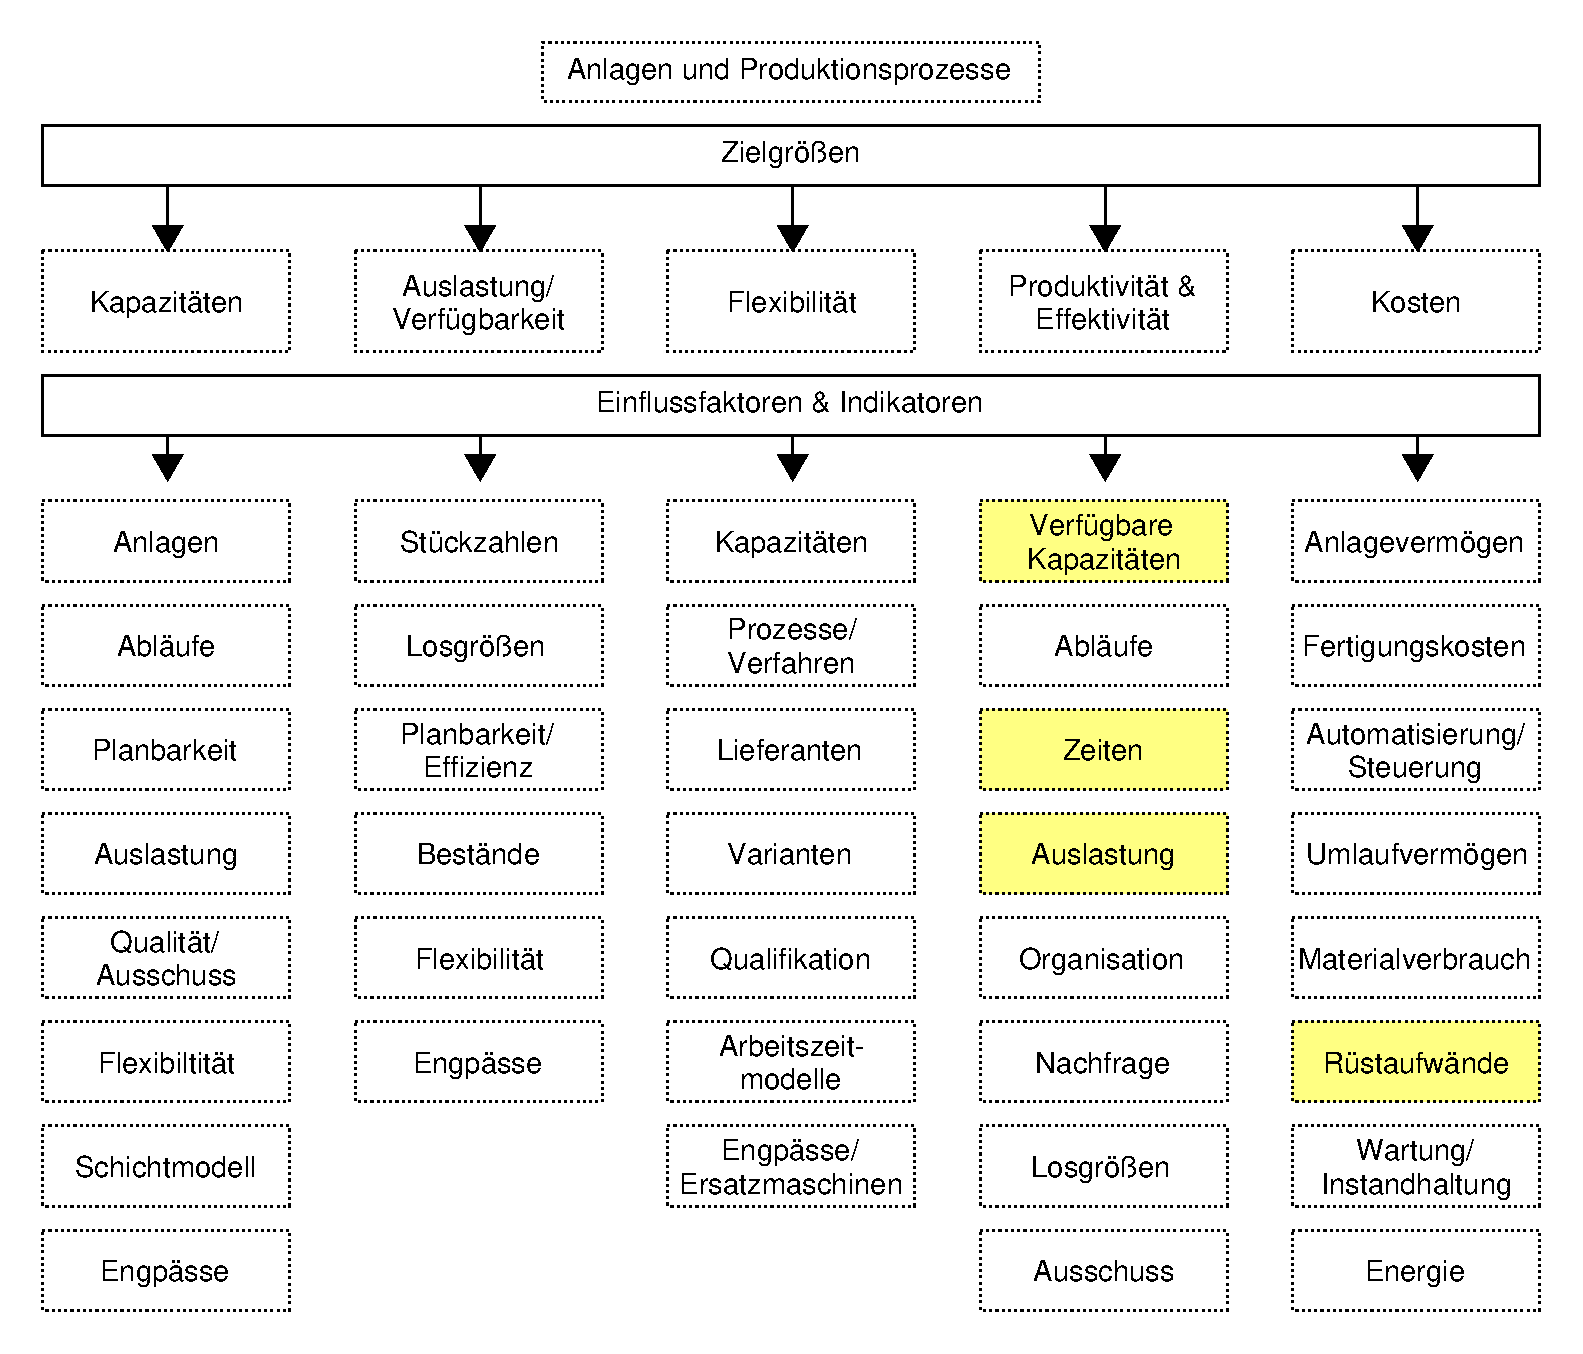
\includegraphics[scale=0.5]{DA_files/Bilder/Analyse/Produktionsprozesse-Zielgroessen.pdf}
\caption{Produktionsprozess: Zielgrößen und Einflussfaktoren}
\label{pic:Produktionsprozesse-Zielgroessen}
\end{figure}

In dieser Arbeiten werden nur einige wenige Einflussfaktoren berücksichtigt. Nicht für jedes Unternehmen und jede Ebene im Unternehmen ist jede Zielgröße und somit auch nicht jeder Einflussfaktor relevant. In dieser Arbeit wird der Fokus im Zuge des Modulaustauschs auf die Ebene der Produktionsplanung und Betriebsleitung gelegt. Auf dieser ist untere anderem die Kapazitätsoptimierung und damit das Ziel der Produktivität \& Effektivität relevant. Die Produktivität beschreibt, wie viel der verfügbaren Arbeitszeit zur Produktion verwendet wird. Steht aufgrund vieler Störungen in der Anlage die Produktion still, so ist die Produktivität gering. Bei einer hohen Effektivität werden die verfügbaren Ressourcen ideal genutzt. Dies kann beispielsweise die Zeit sein, die eine Reparatur in Anspruch nimmt. Folgende Einflussfaktoren sollen im weiteren Verlauf der Arbeit berücksichtigt werden:
\begin{itemize}
\item \textbf{Zeiten:} Wie viel Stillstandzeit verursacht der Modulaustausch?
\item \textbf{Auslastung:} Besteht die Möglichkeit vor zu produzieren?
\item \textbf{Rüstaufwände:} Was muss alles im Rezept verändert werden? Welche Zeit nimmt das in Anspruch?
\item \textbf{Verfügbare Kapazitäten:} Wie viele Mitarbeiter stehen für den Modultausch zur Verfügung? 
\end{itemize}

\section{Informationsanpassung}
Die Individualisierung von Software bietet die Möglichkeit eine Vielzahl von Nutzer und Aufgaben zu unterstützen. Individualisierung dient der Modifizierung von Interaktion und Informationsdarstellung, um unter anderem den Fähigkeiten und Bedürfnissen jedes Benutzers gerecht zu werden. Ebenso ist auch die Anpassung an das zu lösende Problem nicht zu unterschätzen. Je nach Zielstellung müssen andere Informationen hervor gehoben werden.

\subsection{Individualisierung für den Menschen}
Individualisierung für den Nutzer kann vielschichtig sein. In Abschnitt \ref{2:Individualisierung} sind bereits einige Aspekte für Individualisierung thematisiert. Zu Berücksichtigen sind bei Sicht auf den Nutzer unter anderem:
\begin{itemize}
\item \textbf{Fähigkeiten:} Welche besonderen Fähigkeiten hat der Nutzer? Wie können diese in Kollaboration mit der Assistenz sinnvoll genutzt werden?
\item \textbf{Vorwissen:} Was weiß der Nutzer über die modulare Anlage?
\item \textbf{Position:} Welche Aufgabe hat der Nutzer? Auf welcher Ebene des Unternehmens arbeitet dieser? Welche Informationen sind für ihn besonders relevant?
\end{itemize}
Soll jeder Nutzer des Assistenzsystemes individuell anhand seiner kognitiven Leistung unterstützt werden, so ist herauszufinden, ob der Mensch aktuell mit der Aufgabe über- oder unterfordert ist. Eine Möglichkeit ist die Art und Weise der Interaktion auszuwerten und entsprechende Anpassungen vorzunehmen. Wie bereits in Abschnitt \ref{2:Adaptive-Systeme} beschrieben, sind dabei viele Einflussfaktoren zu berücksichtigen. Eine Auswertung dieser sprengt leider den Rahmen der Arbeit. \todo{Was schaue ich mir an?}

\subsection{Anpassung an die Aufgabe}
\label{3:Anpassung-Aufgabe}
Wie schon in Abschnitt \ref{2:Unterscheidung-Probleme} beschrieben, lassen sich Probleme anhand verschiedener Aspekte unterscheiden. So ist zum Beispiel der Zeitdruck ein wichtiger Aspekt. Bei zeitkritischen Problemen muss möglichst schnell eine gute Lösung gefunden werden. Ist das Problem nicht zeitkritisch, können in Ruhe alle zur Verfügung stehenden Informationen in den Problemlöseprozess mit einbezogen werden. So kann bei einem zeitkritischen Problem ein höherer Automatisierungsgrad gefordert sein. Um dennoch dem Menschen seine Kompetenzen nicht abzusprechen, ist es möglich bei Problemen, die eher langfristig sind und die eine höhere kognitive Aktivität erfordern, eine geringere Autonomiestufe anzuwenden. Dadurch kann der Mensch sich Wissen über den Prozess aneignen und seine Kompetenzen ausbauen.

Angenommen der Nutzer hat viel Zeit sich mit dem Problem zu beschäftigen, so müssen sich die bereitgestellten Informationen auch am Probleminhalt orientieren. Der Austausch eines Moduls bedarf einer Übersicht der Kompatibilität mit der bestehenden Anlage und dem Rezept. Entsteht ein Problem aufgrund eines fehlgeschlagenen Services, so ist das zugehörige Equipment und die eingestellten Parameter relevant. Durch die Aufbereitung dieser Informationen und deren Abhängigkeiten kann schrittweise die Ursache gefunden werden.

Ein ebenfalls wichtiger Aspekt, der schon in Abschnitt \ref{3:Informationsbedarf-Operator} thematisiert wurde, ist die Zielsetzung des Unternehmens. Diese kann sehr unterschiedlich sein, was sich maßgeblich auf die Informationsbereitstellung auswirkt. Ist beispielsweise die Stillstandzeit der Anlage besonders relevant, so sollten diese Informationen hervor gehoben werden. In einem anderen Kontext kann aufgrund von Personalmangel der Rüstaufwand eine höhere Priorität bekommen.

\section{Interaktionsmechaniken}
\todo{weiter ausführen, Vor- und Nachteile}
Im Kontext dieser Arbeit wird das Problemlösen betrachtet. Problemlösen heißt in diesem Fall aus mehreren Alternativen die geeignetste für das Erreichen des festgelegten Ziels auszuwählen. In Abschnitt \ref{2:Assistenzsysteme} sind verschiedene Interaktionsmechaniken beschrieben. Um diese geeignet bewerten zu können ist zunächst eine Begutachtung des Arbeitsumfelds und der Aufgaben notwendig.

Da sich das Problemlösen im Rahmen dieser Arbeit nicht auf das Beheben von Störungen bezieht, kann angenommen werden, dass die Hände nicht für andere Aufgaben frei sein müssen. Zudem ist eine geeignete Darstellung von Zusammenhängen notwendig, welches eine entsprechende Displaygröße voraussetzt. Diese Zusammenhänge müssen durch den Menschen entsprechend interpretiert werden, damit dieser mit dem System interagieren kann. Es muss dazu die Möglichkeit gegeben sein selbst Vorschläge für die Lösung des Problems zu liefern. Das setzt vielfältige Eingabemöglichkeiten voraus. \todo{spezifizieren!}

Daraus abgeleitet wird für die Umsetzung des Assistenzsystem ein Tablet verwendet. Diese ist groß genug, um alle notwendigen Informationen anzuzeigen. Es ist flexibel genug, wenn für den Problemlöseprozess Informationen benötigt werden, die nur durch Begutachtung der Anlage erlangt werden können. Zudem bietet die Kamera die Möglichkeit Augumented Reality zu verwenden oder das Mikrofon die Möglichkeit Spracheingaben zu tätigen.



\section{Anforderungen an das Assistenzsystem}
\label{3:Anforderungen}

\subsection{Funktionale Anforderungen}

\subsubsection*{Unterstützung der Problemidentifikation}
\begin{itemize}
\item[PI 1] Der Nutzer soll durch die Problemlösung begleitet werden können, indem...
	\begin{itemize}
	\item[PI 1.1] ...er das Problem beschreiben kann.
	\item [PI 1.2] ...er Ziele definieren kann.
	\item[PI 1.3] ...ihm alle Informationen über die aktuelle Situation zur Verfügung stehen.
	\end{itemize}
\item[PI 2] Das Assistenzsystem soll den Nutzer bei der Problemidentifikation unterstützen.
\item[PI 3] Dem Nutzer soll es möglich sein Ziele hinzuzufügen.
\item[PI 4] Dem Nutzer soll der Auslöser des Problems und der zugehörige Problembereich mitgeteilt werden.
\end{itemize}

\subsubsection*{Unterstützung bei der Problemlösung}
\begin{itemize}
\item[PL 1] Das Assistenzsystem soll mögliche Lösungen vorschlagen.
	\begin{itemize}
	\item[PL 1.1] Diese sollen sich an den festgelegten Zielen orientieren.
	\end{itemize}
\item[PL 2] Der Nutzer soll mögliche Lösungen vorschlagen können.
\item[PL 3] Die Lösungen sollen vergleichbar sein, indem...
	\begin{itemize}
	\item[PL 3.1] ...die Auswirkungen auf die Anlage/ den Prozess dargestellt werden.
	\item[PL 3.2] ...die verschiedene Einflussfaktoren sichtbar sind.
	\end{itemize}
\item[PL 4] Die Lösungen sollen bewertbar sein.
\end{itemize}

\subsubsection*{Kluster von Problemen}
\begin{itemize}
\item[KP 1] Es sollen mehrere Probleme gleichzeitig bearbeitet werden können.
\item[KP 2] Die Probleme sollen sich sortieren lassen.
\item[KP 3] Die Probleme sollen mit Merkmalen versehen werden.
	\begin{itemize}
	\item[KP 3.1] Zeit: Bis wann muss das Problem gelöst sein?
	\item[KP 3.2] Komplexität: Wird die Problemlösung durch viele oder wenige Größen beeinflusst?
	\item[KP 3.3] Arbeitsaufwand: Anzahl der Arbeitsstunden
	\end{itemize}
\end{itemize}

\subsection{Nichtfunktionale Anforderungen}
\begin{itemize}
\item[NA 1] Die Bedienung soll über ein Tablet realisiert werden.
\end{itemize}
